
\section{3D Visualization}
\label{sec:viz}
You will now create a 3D visualization of the temple images. By treating our two images as a stereo-pair, we can triangulate corresponding points in each image, and render their 3D locations.

\subparagraph*{Q4.1}\points{15} In \texttt{q4\_1\_epipolar\_correspondence.py} finish the function \\ \texttt{epipolarCorrespondence} with the signature:
\begin{center}
    \texttt{[x2, y2] = epipolarCorrespondence(im1, im2, F, x1, y1)}
\end{center}
This function takes in the $x$ and $y$ coordinates of a pixel on \verb!im1! and your fundamental matrix $\F$, and returns the coordinates of the pixel on \verb!im2! which correspond to the input point. The match is obtained by computing the similarity of a small window around the $(x_1, y_1)$ coordinates in \verb!im1! to various windows around possible matches in the \verb!im2! and returning the closest.

Instead of searching for the matching point at every possible location in \verb!im2!, we can use $\F$ and simply search over the set of pixels that lie along the epipolar line (recall that the epipolar line passes through a single point in \verb!im2!  which corresponds to the point $(x_1, y_1)$ in \verb!im1!).

There are various possible ways to compute the window similarity. For this assignment, simple methods such as the Euclidean or Manhattan distances between the intensity of the pixels should suffice.  See \cite{szeliski2022computer} chapter 11, on stereo matching, for a brief overview of these and other methods.

\textbf{\emph{Implementation hints:}}
\begin{itemize}
    \item Experiment with various window sizes.
    \item It may help to use a Gaussian weighting of the window, so that the center has greater influence than the periphery.
    \item Since the two images only differ by a small amount, it might be beneficial to consider matches for which the distance from $(x_1, y_1)$ to $(x_2, y_2)$ is small.
\end{itemize}
To help you test your \texttt{epipolarCorrespondence}, we have included a helper function \texttt{epipolarMatchGUI} in \texttt{q4\_1\_epipolar\_correspondence.py}, which takes in two images and the fundamental matrix. This GUI allows you to click on a point in \texttt{im1}, and will use your function to display the corresponding point in \texttt{im2}. See \autoref{fig:epigui2}.
\begin{figure}[h]
    \centering
    \fbox{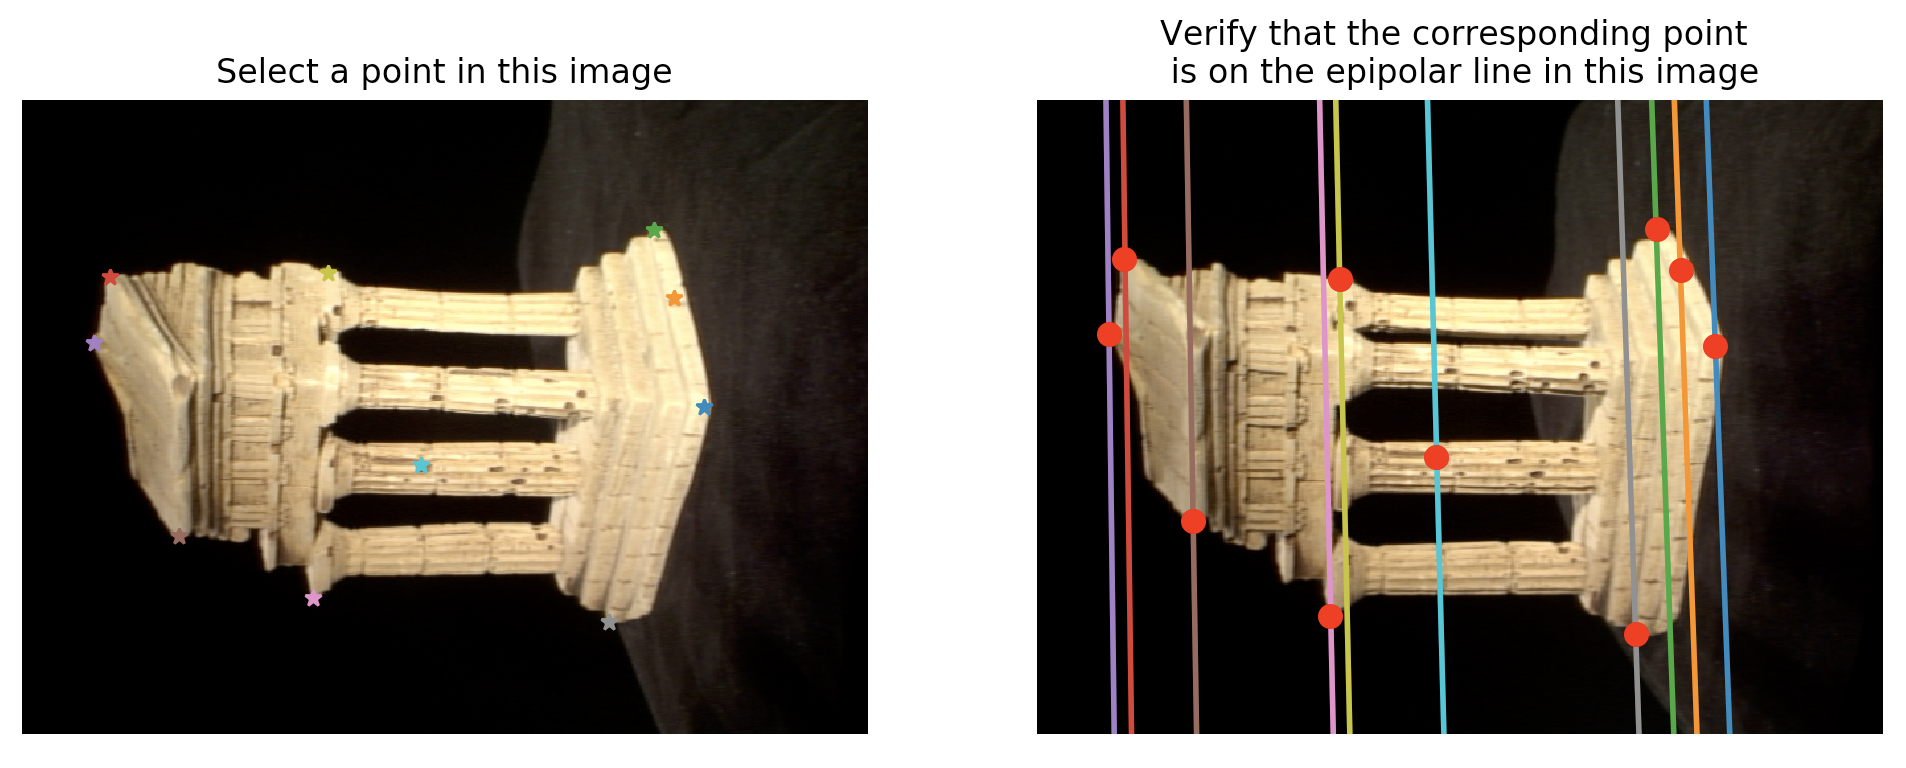
\includegraphics[width=0.8\textwidth]{images/q3gui_disp_arun.png}}
    \caption{\texttt{epipolarMatchGUI} shows the corresponding point found by
    calling \texttt{epipolarCorrespondence}}
    \label{fig:epigui2}
\end{figure}

It's not necessary for your matcher to get \textit{every} possible point right, but it should get easy points (such as those with distinctive, corner-like windows). It should also be good enough to render an intelligible representation in the next question.

\deliver{
\textbf{Output:} Save the matrix $\F$, points \texttt{pts1} and \texttt{pts2} which you used to generate the screenshot to the file \texttt{q4\_1.npz}. 

\textbf{In your write-up:} 
\begin{itemize}
    \item Include a screenshot of \texttt{epipolarMatchGUI} with some detected correspondences.
    \item Include the code snippet of \texttt{epipolarCorrespondence} function.
\end{itemize}
}

\begin{your_solution}[title=Q4.1,height=9cm,width=\linewidth]
The following \autoref{fig:Q4_1_result} shows the screenshot of epipolarMatchGUI() with some detected correspondences using the epipolarCorrespondence() function:
\newline
\begin{minipage}{1\linewidth}
	\centering
	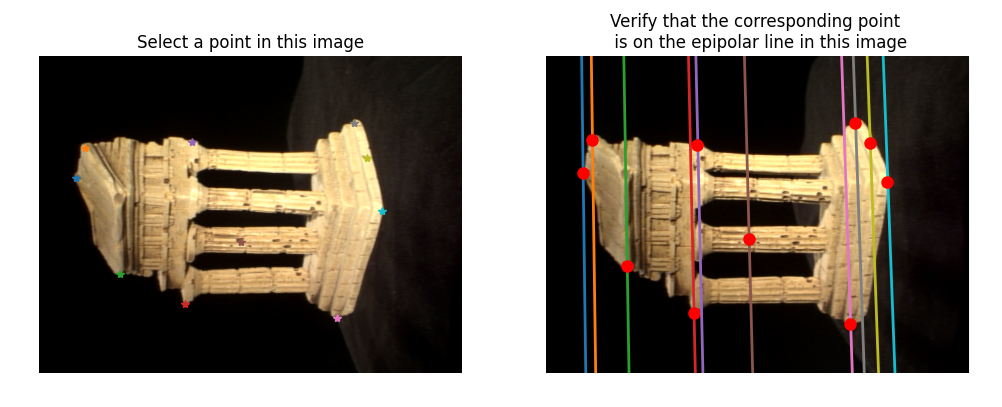
\includegraphics[width=1\linewidth, height=0.39\columnwidth]{../Q4_1_result.png}
	\refstepcounter{figure}  % Increment the figure counter
	\textbf{Figure \ref{fig:Q4_1_result}:} Result of the epipolarCorrespondence() Function  % Manually add a caption/title
	\label{fig:Q4_1_result}         % Label for referencing	
\end{minipage}
\end{your_solution}
\newpage
\begin{your_solution}[title=Q4.1 continued,height=21.5cm,width=\linewidth]
	The following \autoref{fig:Q4_1_cns} shows the code snippet of the epipolarCorrespondence() function in q4\_1\_epipolar\_correspondence.py:	
	\newline
	
	
	\begin{minipage}{1\linewidth}
		\centering
		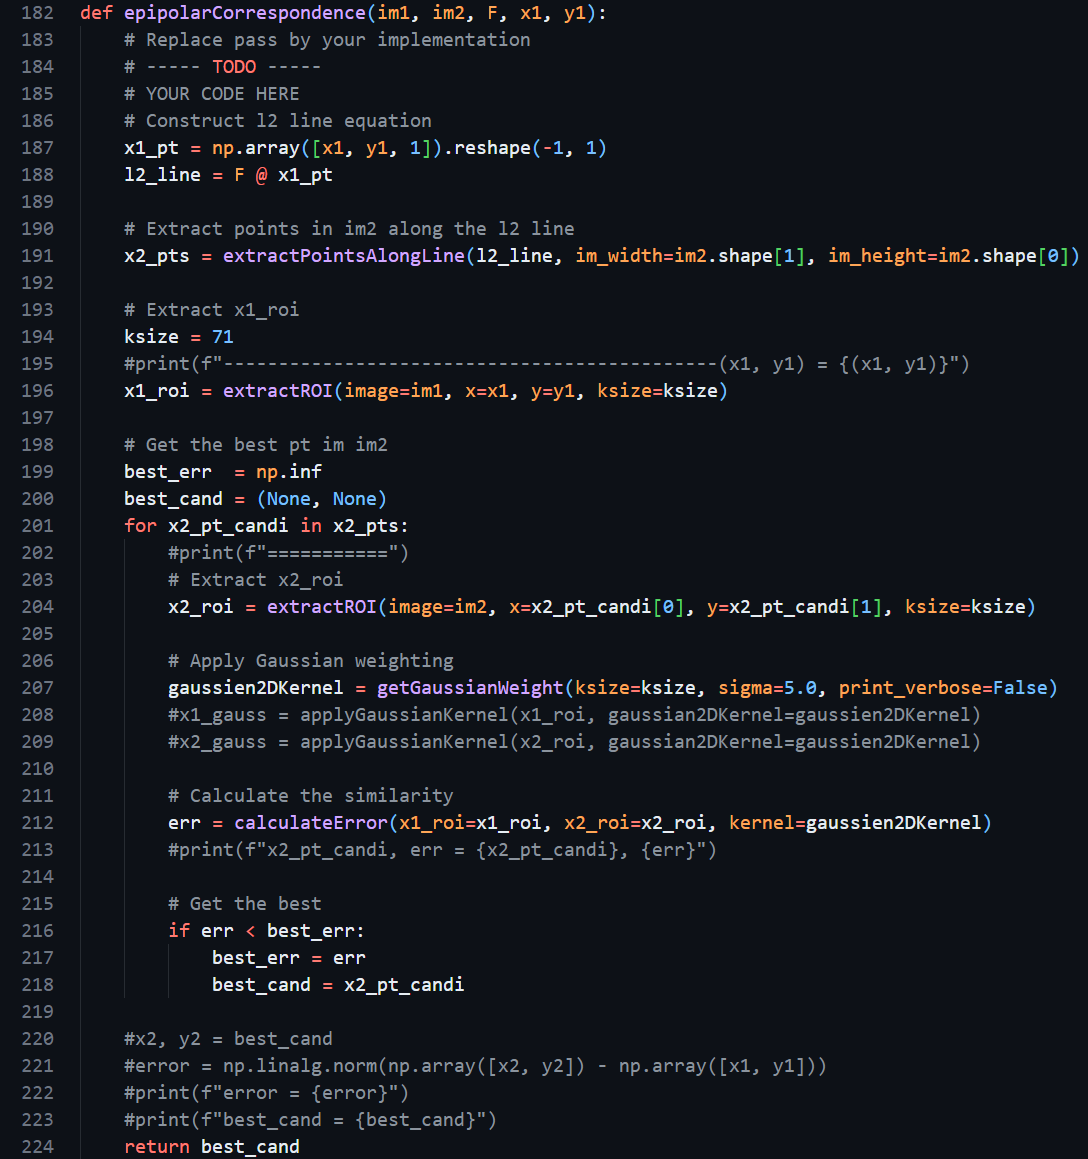
\includegraphics[width=1\linewidth, height=1.2\columnwidth]{../Q4_1_cns.png}
		\refstepcounter{figure}  % Increment the figure counter
		\textbf{Figure \ref{fig:Q4_1_cns}:} Code Snippet of the epipolarCorrespondence() Function  % Manually add a caption/title
		\label{fig:Q4_1_cns}         % Label for referencing	
	\end{minipage}
\end{your_solution}

\subparagraph*{Q4.2}\points{10}
Included in this homework  is a file \texttt{data/templeCoords.npz} which contains 288 hand-selected points from \verb!im1! saved in the variables \verb!x1! and \verb!y1!.

Now, we can determine the 3D location of these point correspondences using the \texttt{triangulate} function. These 3D point locations can then be plotted using the Matplotlib or plotly package. Complete the \texttt{compute3D\_pts} function in \texttt{q4\_2\_visualize.py}, which loads the necessary files from \texttt{../data/} to generate the 3D reconstruction using \texttt{scatter} function matplotlib. An example is shown in \autoref{fig:q3}. 
\begin{figure}[t]
    \centering
    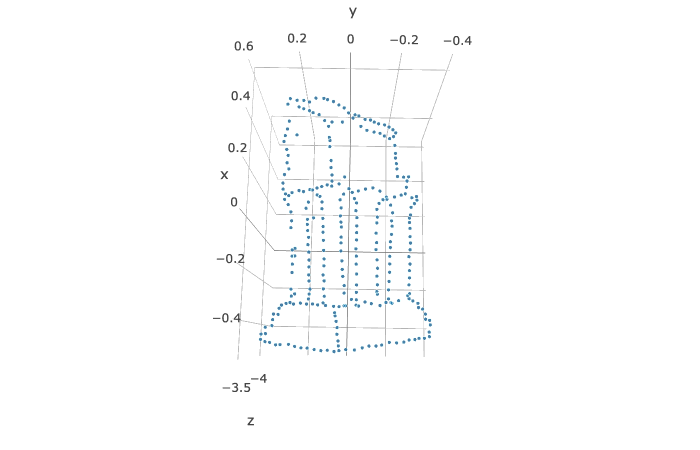
\includegraphics[width=0.4\textwidth]{images/q3a.png}
    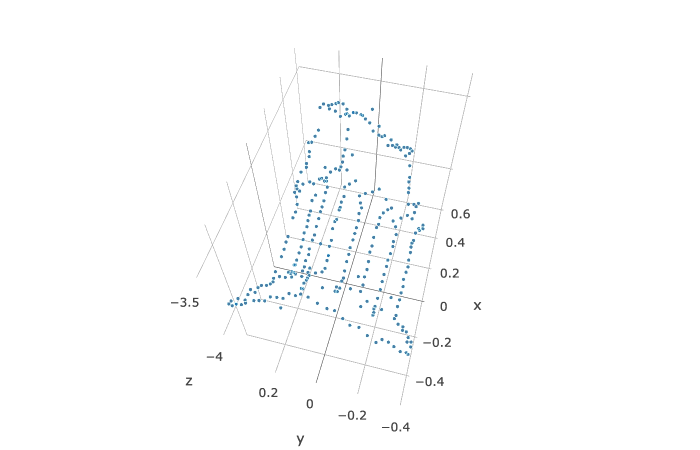
\includegraphics[width=0.4\textwidth]{images/q3b.png}\\
    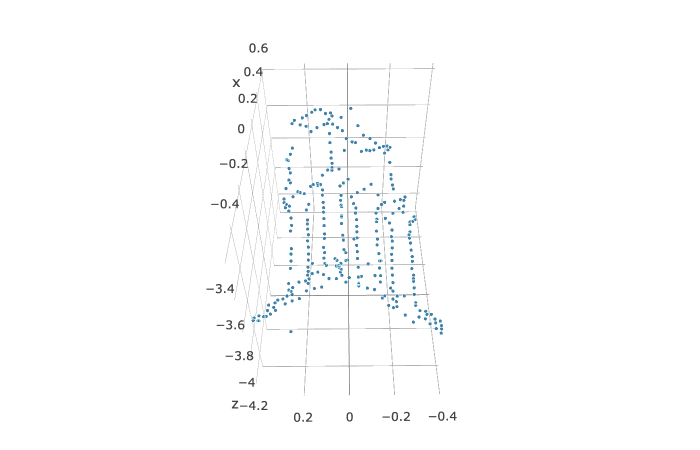
\includegraphics[width=0.4\textwidth]{images/q3c.png}
    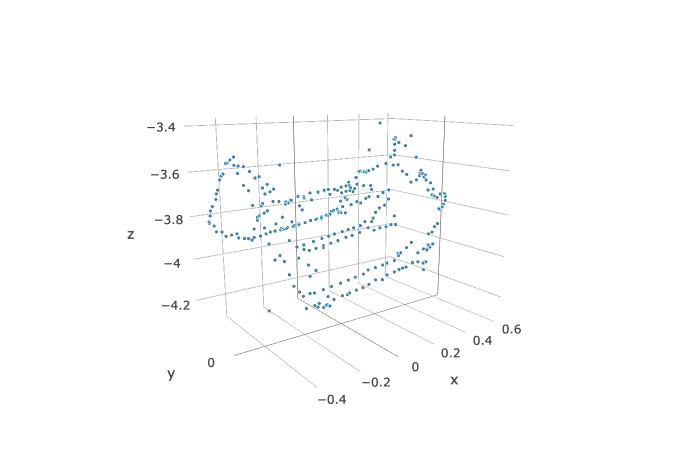
\includegraphics[width=0.4\textwidth]{images/q3d.png}
    \caption{An example point cloud}
    \label{fig:q3}
\end{figure}

\deliver{
\textbf{Output:} Again, save the matrix $\F$, matrices $\M1, \M2, \C1, \C2$ which you used to generate the screenshots to the file \texttt{q4\_2.npz}. 

\textbf{In your write-up:} 
\begin{itemize}
    \item Take a few screenshots of the 3D visualization so that the outline of the temple is clearly visible, and include them in your writeup.
    \item Include the code snippet of \texttt{compute3D\_pts} function in your write-up. 
\end{itemize}
}

\begin{your_solution}[title=Q4.2,height=17.5cm,width=\linewidth]
The following \autoref{fig:Q4_2_sh1}, \autoref{fig:Q4_2_sh2}, \autoref{fig:Q4_2_sh3} and \autoref{fig:Q4_2_sh4} show the results of the 3D visualization results of the temple:
\newline

\begin{minipage}{0.55\linewidth}
	\centering
	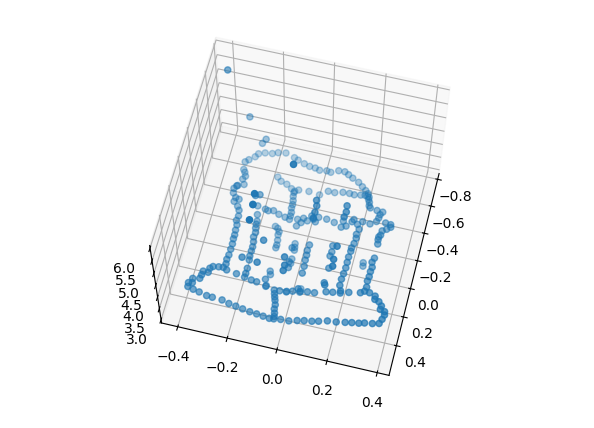
\includegraphics[width=\linewidth]{../Q4_2_sh1.png}
	\refstepcounter{figure}  % Increment the figure counter
	\textbf{Figure \ref{fig:Q4_2_sh1}:} First Screenshot  % Manually add a caption/title
	\label{fig:Q4_2_sh1}         % Label for referencing	
\end{minipage}
\hfill
\begin{minipage}{0.45\linewidth}
	\centering
	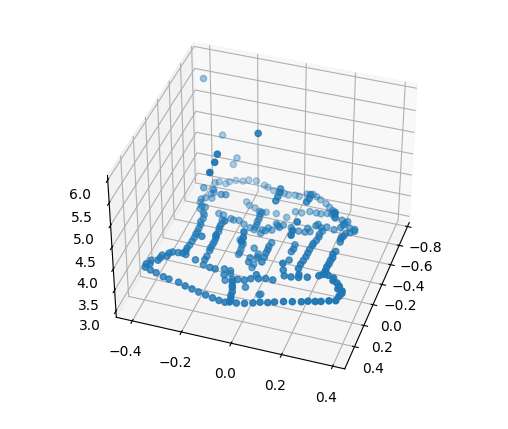
\includegraphics[width=\linewidth]{../Q4_2_sh2.png}
	\refstepcounter{figure}  % Increment the figure counter
	\textbf{Figure \ref{fig:Q4_2_sh2}:} Second Screenshot  % Manually add a caption/title
	\label{fig:Q4_2_sh2}         % Label for referencing
\end{minipage}	
\newline
\begin{minipage}{0.45\linewidth}
	\centering
	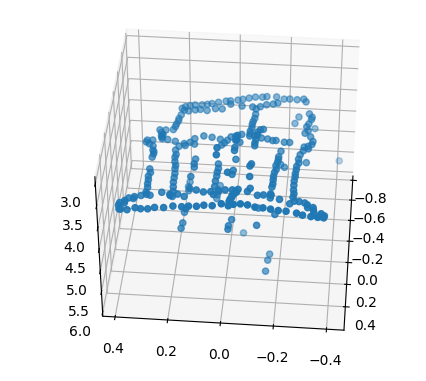
\includegraphics[width=\linewidth]{../Q4_2_sh3.png}
	\refstepcounter{figure}  % Increment the figure counter
	\textbf{Figure \ref{fig:Q4_2_sh3}:} Third Screenshot  % Manually add a caption/title
	\label{fig:Q4_2_sh3}         % Label for referencing	
\end{minipage}
\hfill
\begin{minipage}{0.55\linewidth}
	\centering
	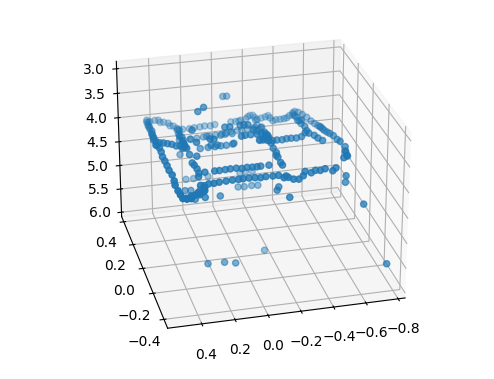
\includegraphics[width=\linewidth]{../Q4_2_sh4.png}
	\refstepcounter{figure}  % Increment the figure counter
	\textbf{Figure \ref{fig:Q4_2_sh4}:} Fourth Screenshot  % Manually add a caption/title
	\label{fig:Q4_2_sh4}         % Label for referencing
\end{minipage}	
\end{your_solution}
\newpage
\begin{your_solution}[title=Q4.2 continued,height=18.5cm,width=\linewidth]
	The following \autoref{fig:Q4_2_cns} shows the code snippet of the compute3D\_pts() function in q4\_2\_visualize.py:	
	\newline
	
	
	\begin{minipage}{1\linewidth}
		\centering
		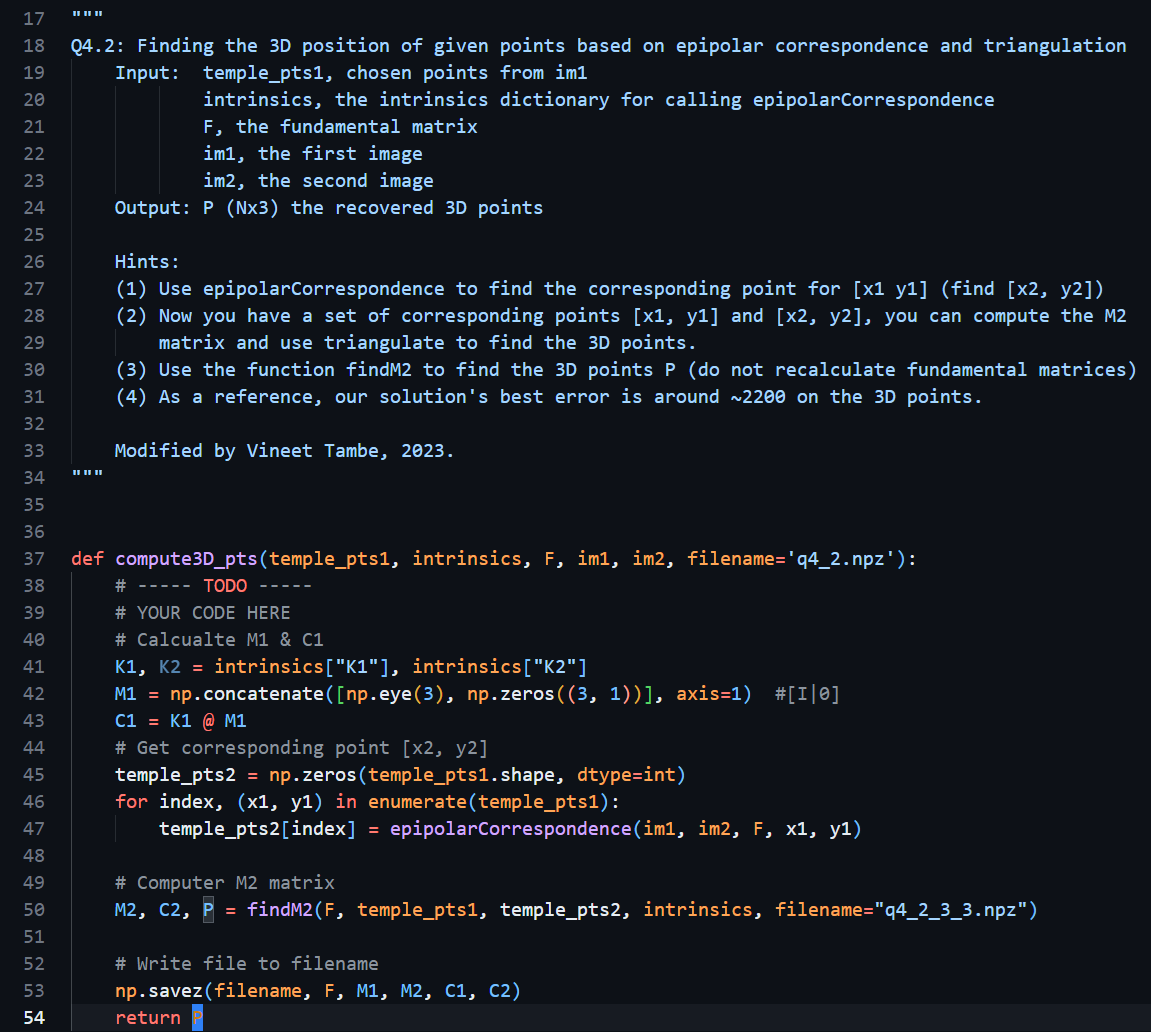
\includegraphics[width=1\linewidth, height=1\columnwidth]{../Q4_2_cns.png}
		\refstepcounter{figure}  % Increment the figure counter
		\textbf{Figure \ref{fig:Q4_2_cns}:} Code Snippet of the compute3D\_pts() Function  % Manually add a caption/title
		\label{fig:Q4_2_cns}         % Label for referencing	
	\end{minipage}
\end{your_solution}